% Chapter Template

\chapter{Introduction} % Main chapter title

\label{Chapter 1} % Change X to a consecutive number; for referencing this chapter elsewhere, use \ref{ChapterX}

\lhead{Chapter 1. \emph{Introduction}} % Change X to a consecutive number; this is for the header on each page - perhaps a shortened title

%----------------------------------------------------------------------------------------
%	SECTION 1
%---------------------------------------------------------------------------------------
\section{Introduction}
    The rise of parallel programming languages like OpenCL \cite{stone2010opencl}, CUDA \cite{nvidia} and widespread availability of heterogeneous computing platforms comprising CPUs and GPUs have paved the way for researchers to develop efficient scientific computing workloads spanning across diverse domains of science. In the past few years, both of these heterogeneous programming languages have been extensively used for developing high performance computing (HPC) applications for execution on heterogeneous multicore architectures ranging from cluster level workstations to heterogeneous embedded platforms comprising multiple CPUs and GPUs. Both frameworks support asynchronous event driven programming models that enable both data parallel and task parallel paradigms of computation for implementing high performance parallel applications. The data parallel programming model has provisions for implementing a computational kernel which represents the core computation for a given algorithm. A data parallel computational kernel launches multiple threads in parallel across multiple SIMD enabled compute units. Each thread applies the specified kernel  transformation to designated data points of the input data space. The task parallel programming model supports parallelism at the task/kernel level where application task graphs comprising multiple kernels with dependencies, each representing distinct computational transformations can be dispatched and executed on  multiple devices in a target heterogeneous platform. The OpenCL runtime system additionally has provision for program portability across different types of devices i.e. the same computational kernel source code can be compiled into device specific binaries for execution on different devices.
    
	 Given heterogeneous platforms comprising multiple devices of varying computational power, determining efficient architecture-to-application mapping decisions require extensive domain knowledge of platform level characteristics as well as precedence constraints enforced by the application task graph. As an illustrative example, let us consider a simple fork-join task graph in Figure \ref{fig:dagmapping}.
	\begin{figure}[ht] 
		\centering
		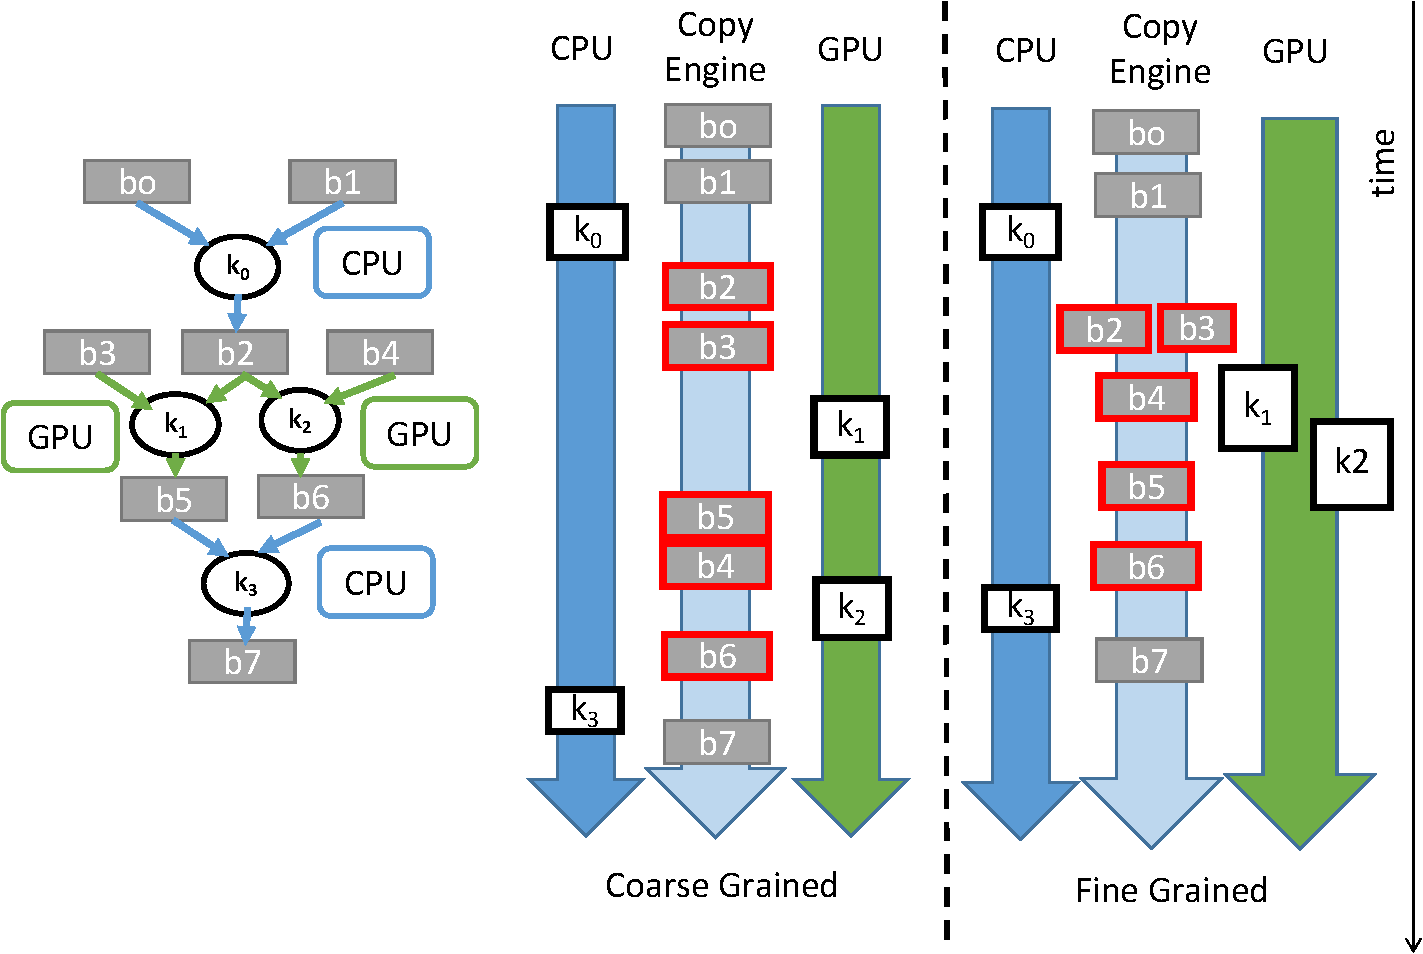
\includegraphics[scale=0.35]{Pictures/TC_IntroPicNew.pdf}
		\caption{DAG Mapping Decisions \label{fig:dagmapping}}
    \end{figure}  
    
    We consider a heterogeneous platform comprising a single CPU and a single GPU along with a DMA copy engine responsible for transferring data across the PCI-Express bus from the CPU to the GPU and back. The fork-join graph comprises four tasks, each representing some computational kernel which takes as input two input buffers and produces one output buffer. In Fig. \ref{fig:dagmapping}, the rectangular nodes represent input output buffers and the circular nodes represent kernels. We use this convention throughout the paper. The edges between a buffer and task represents the precedence constraints between tasks as well. Given a heterogeneous compute platform comprising a single CPU and a single GPU there can exist a total of 16 task-device mappings for this task graph where task(s) are  either mapped to a GPU device or a CPU device. In Fig. \ref{fig:dagmapping}, we explore one of the 16 possible mappings where $k_0$ and $k_3$ are  mapped to a CPU device, $k_1$ and $k_2$ are mapped to a GPU device. 

    Scheduling decisions for general application DAGs are coarse-grained - each task is mapped to a single device at a time and the associated kernel execution, buffer reads and writes are finished completely before proceeding to execute successors of the kernels. In Fig. \ref{fig:dagmapping}, for kernel $k_2$ to start execution, $k_1$ must finish and the copy engine should copy the resultant buffer $b_5$ to the host. After that the required input buffer $b_4$ has to be copied to the GPU device. The scheduling decisions are achieved by designing complex host programs that orchestrate the process of mapping individual kernels to target devices of the heterogeneous platform while maintaining precedence constraints. Alternatively, there exist several frameworks proposed in the recent past that alleviate the burden of implementing such complex orchestrators for undertaking coarse-grained scheduling decisions. The frameworks can be classified into two broad categories - i) frameworks like \cite{pekka,henry2014toward} that provide either a top-level API or additional programming constructs using which an end designer has to modify existing OpenCL benchmark source code and ii) frameworks such as StarPU, MultiCL that provides scheduling engines  \cite{augonnet2011starpu,multicl} optimized for heterogeneous clusters with support for custom scheduling heuristics for mapping a dataflow graph of OpenCL kernels on a heterogeneous platform. Both styles rely on deriving coarse-grained scheduling decisions for application DAGs. 

    In contrast, we believe scheduling decisions should be more fine-grained in nature allowing execution of multiple tasks in the same device and interleaving copy operations with execute operations. This is exemplified in the right hand side scheduling option of Fig. \ref{fig:dagmapping}. We can observe for kernel $k_1$, the two input buffers $b_2$ and $b_3$ can be transferred by the copy engine in parallel. Also while kernel $k_1$ is executed,  $b_4$ can be transferred asynchronously to the GPU device. The kernel $k_2$ executes in parallel with $k_1$ while sharing the same GPU resource. As a result, we observe that the individual times of $k_1$ and $k_2$ increase. However, the overall time to finish DAG execution decreases. 

    Implementing such fine-grained scheduling requires designing an even more complex host program capable of  i) asynchronously interleaving data transfers as and when required and ii) clustering multiple tasks to the same device as and when feasible. These scheduling decisions can be achieved by setting up multiple worker queues per device and asynchronously enqueueing commands for executing multiple kernels on the same device. For the CUDA runtime system, these worker queues are referred as {\em CUDA streams}.  For the OpenCL runtime these are referred as {\em command queues}. Naturally, the end user has to consider the computational capability of the device and the individual computational requirements of each concurrent kernel before dispatch. 

    We propose {\em PySchedCL} a platform agnostic programming framework which is possibly the first computer-aided design solution that is capable of automating the process of deriving both coarse-grained and fine-grained scheduling decisions for efficient collaborative execution of application task graphs on heterogeneous multicores comprising CPU and GPU devices. The proposed framework supports reduction of considerable implementation overhead and automatically outputs scheduling decisions that exploit concurrency with minimal intervention by the programmer. The framework is built using the widely used PyOpenCL API \cite{pyopencl} and facilitates rapid development and deployment of OpenCL applications. We choose OpenCL, since it offers device portability, thus supporting a myriad of heterogeneous compute devices such as CPU, GPUs, FPGAs, DSPs etc. Our framework enables the user to concentrate only on developing OpenCL kernels and providing minimum guidance parameters that would help in finally determining near optimal runtime scheduling decisions for data parallel applications on a target heterogeneous CPU-GPU platform. We note the optimizations proposed are generic and the ideas can be leveraged for any data parallel heterogeneous setting. The salient features of the proposed framework are enumerated as follows.

\begin{itemize}
    \item The framework supports a design frontend that will facilitate programmers to develop and execute application task graphs without having to consider the intricacies of runtime environment. The frontend has provisions for a specification file using which the programmer can construct the input specification for each OpenCL kernel in the task graph as well as provide  precedence constraints.  The task of the application designer is only to develop individual kernels and populate these specification files.
    \item The framework supports a scheduling engine which automatically issues directives required by the OpenCL runtime system for executing an application comprising either a single kernel or multiple kernels with dependencies efficiently. This completely bypasses the the requirement of manually writing a host program which captures all low level scheduling decisions. The scheduling engine  mimics the behaviour of the orchestrating host program and has support for clustering kernels in a task graph as well as automatically making decisions that involve concurrent kernel execution on the same device.
    \item In addition to the modules above, the framework has provisions for specifying guidance parameters using which the framework can automatically set up device worker queues that can exploit application level concurrency on heterogeneous compute platforms. We showcase the efficacy of this approach by considering a inference pipeline for the Transformer Nerual Network architecture \cite{DBLP:journals/corr/VaswaniSPUJGKP17} which is an application that provides ample scope for concurrency and parallelization. We provide extensive experimental results for the same comparing our approaches with standard dynamic list scheduling algorithms provided in frameworks such as StarPU \cite{augonnet2011starpu}, SOCL \cite{henry2014toward} etc. The static fine-grained scheduling approach exhibits  speedups in the range of $1.4-3.4x$ when compared to the dynamic coarse-grained scheduling approaches.     
\end{itemize}

The framework thus eases complex OpenCL application development with the help of specification files and automatically exploits available fine/coarse grained scheduling techniques for mapping data-computational kernels to OpenCL compliant devices in an heterogeneous CPU-GPU platform. 
\par Chapter \ref{Chapter2} presents necessary background and domain knowledge of the OpenCL runtime system and support offered by existing frameworks. Chapter \ref{Chapter3} details the motivation behind the design of this framework and a formal presentation of the problem statement. Chapter \ref{Chapter4} follows it up by outlining the software architecture  and the details of the various components of the framework . Chapter \ref{Chapter5} provides a description of the various scheduling heuristics (both fine and coarse grained) on which we have performe extensive experimentation. We provide a comparative evaluation between these approaches in Chapter \ref{Chapter6}. 
   
